\section{Motivation} % p 2.5
    Clinical diagnostics and research has been improved dramatically with emergence of volumetric imaging such a as \ac{CT} and \ac{MRI} technology which enables visualizing body parts and organs.
    Since its invention in xx, the number of acquired \ac{CT} scans has increased xx-fold until 2024. The importance of \ac{MRI} scans, which offer better soft-tissue contrast without exposing radiation to the patient examined \citep{xx}, has likewise increase with now approximately xx million scans taken every year worldwide.
    % Are there some papers that have evidence for benefit of methods?

    Volumetric imaging offers the benefit of capturing the organ of interest unaltered in \ac{3D} space. However, visualizing the \ac{3D} volume is currently still performed on \ac{2D} screens where in case of \ac{CT} and \ac{MRI} a suitable form of \ac{3D} translucent projection for the densly acquired volume has to be found or individual view planes / imaging slices have to be selected for examination. Automated processing is needed in the first case for the visualization itself and in the latter case automated processing can support clinicians navigating the \ac{3D} volume, help classifying organ boundaries, measuring tumour sizes and highlight organ deformations, all of which is complicated to perform manually when navigating a \ac{3D} volume.

    Deep learning with its basic principles invented in the last century, has become a de-facto standard now for automated processing in versatile fields such as for processing text, images, audio, video, analogous signals, biological processes and molecule configurations, agent simulations purely digitally or in combination with sensors and actuators for physical interaction \citep{xx} and has created a significant technology push throughout all of the mentioned areas of application \citep{xx}.
    Of course, this holds true for volumetric medical image analysis as well where formerly hand-crafted method design is now replaced or combined with data-driven, learning-based methods \citep{xx}.

    Deep learning as a form of artificial learning that mimicks the neuronal activity in brain tissue has been found to share some higher-level concepts with human learning as well such as generalization and specialization \citep{xx}.
    Generalization enables the transfer of an experienced stimulus or input to a broader context, whereas specialization narrows generalized concepts down to more individual cases.
    Both processes were first described for fear-learning as a fundamental skill to ensure survival. Over-generalization can lead to anxiety disorders in this regard \citep{xx}, whereas over-specialization can lead to missclassify dangerous situations.

    In deep learning, the ability of models to generalize is a desirable property.  When training deep learning models, over-specialization is an often experienced challenge which is more technically referred to as overfitting and usually undesirable as it limits the performance of trained models for unseen data points \citep{xx}.
    In many technical applications the comparison with survival situations in biological learning may seem drastical, but in medical deep learning this scenario is not too far away, where misinterpretation during automated processing can results in misdiagnosis and potentially impact patients recovery or in the most extreme situations survival.





    % General deep learing findings
    % DL boosted and is boosting performance and outcome in versatile applications. This spans large areas
    % text processing
    % image processing
    % audio processings
    % video processing for robotics
    % robotics itself, sensors actuators
    % analog signals
    % biological processes
    % explorative agent simulations
    % physical applications
    % computer graphics


    % before: spezialized algorithms, frameworks
    % now: models can be used interchangebly with adjustmens to fit the target task at hand.

    % the idea is learning itself - defined as.



    % universal function approximators, but highly dependent on the data as the model itself isnt worth anything before it has been adjusted (trained).
    % AGI - is of recent discussion where some models reach impressive results.



    % this brings us to the term generalization ...
    % Generalization
    % Wholistic models
    % what is needed for learning in the first place?

    % enough data can fit everything

    % still  problems, halluzinations, intransparency,

    % generalization can be tackeled at different stages of the medical image processing pipeline
    % model optimizing?
    % data curation is necessary?

    % can we do sth at training, model application?

    % Medical deep learing findings
    % as well as medical applications and processing of spezialized sensor data such as volumetric data as MRI CT.
    % especially for medical imaging where outcomes can have real world implications on fragile patients.
    % and can also be applied in the medical domain (SAM)

    % advent of deep learning in medical imaging




    % Definition of generalization

    % Gerneralization
    %     Data Acquisition
    %     Data Curation
    %     Model Building
    %     Model Application

    % What has been tried already? in those steps of the pipeline



\section{Objectives} % p 1.5
    % Objectives of this thesis
    % % TODO: What should go here?

    % Examine for all steps of the pipeline how available information / data in medical images can be utilized to improve the outcome

\section{Organisation and Contributions}  % p 3.5

    \begin{figure}
        \label{fig:draft}
        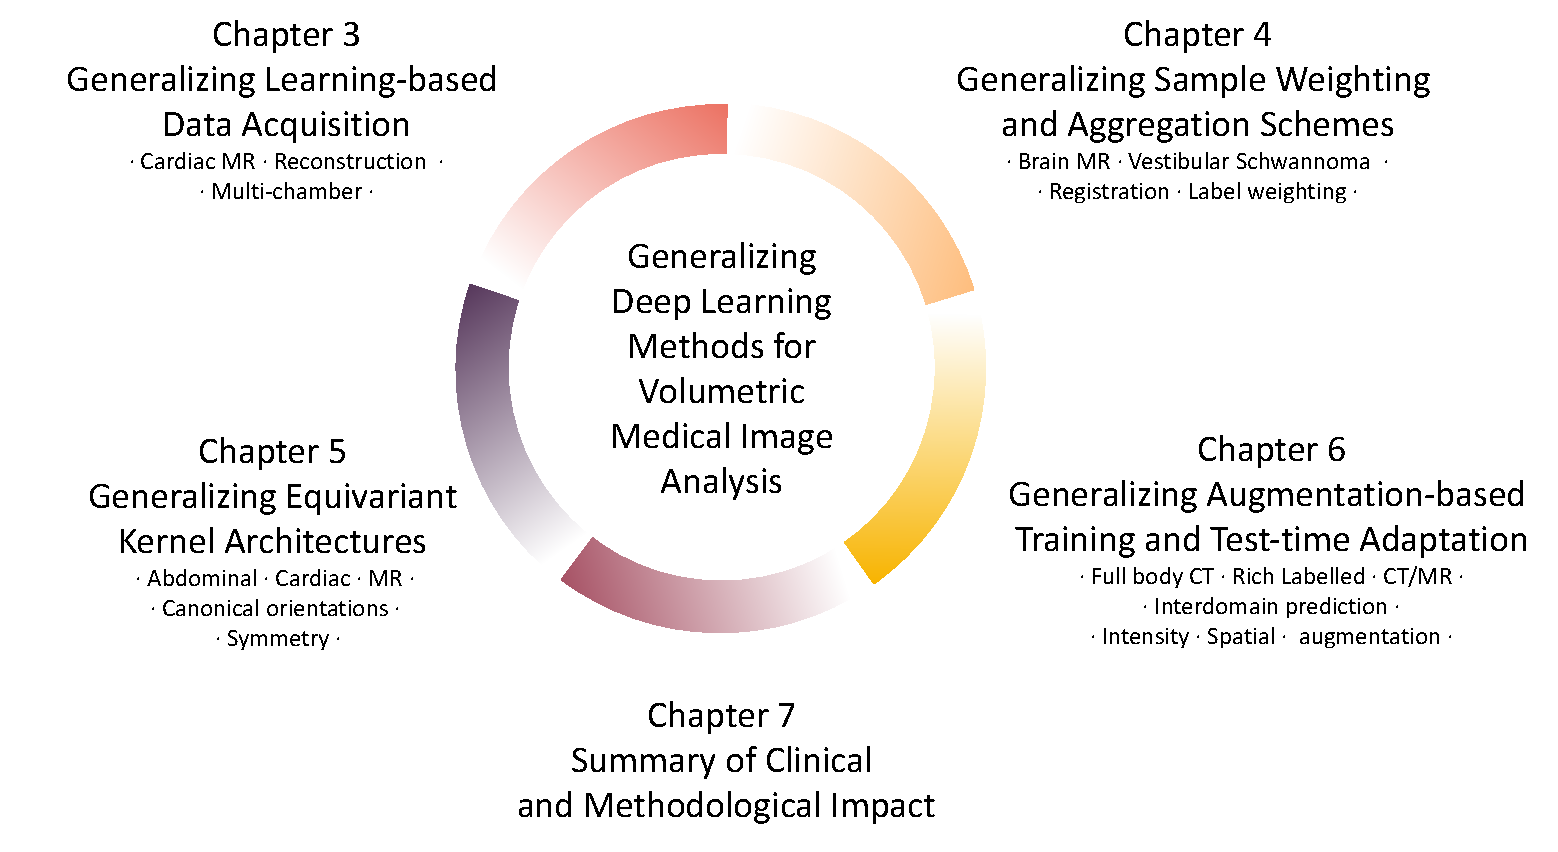
\includegraphics[width=\textwidth]{sections/01_introduction/figures/draft.pdf}
        \caption{Thesis draft}

    \end{figure}